\documentclass[conference]{IEEEtran}
\usepackage{cite}
\usepackage{amsmath,amssymb,amsfonts}
\usepackage{algorithmic}
\usepackage{graphicx}
\usepackage{textcomp}
\usepackage{xcolor}
\usepackage[numbers]{natbib}
\usepackage[normalem]{ulem}
\useunder{\uline}{\ul}{}

\def\BibTeX{{\rm B\kern-.05em{\sc i\kern-.025em b}\kern-.08em
    T\kern-.1667em\lower.7ex\hbox{E}\kern-.125emX}}

\begin{document}
Hello Yunyao,

This is our latest report.

We have some questions we'd like to highlight here.

\begin{itemize}
    \item Do we need to describe the various layers in the transformer encoder layer more in-depth in section \ref{sec:transformer encoder}? Or does our somewhat superficial explanation suffice? 
    \item We are a little unsure about our explanation of the lack of a decoder in our transformer at the end of section \ref{sec:transformer encoder}. Is it good enough?
\end{itemize}

\section{Changelog}
We have made changes to every single section in the paper, and we have also rewritten the transformer section. 
If you have time, please review each section, however, the transformer section is the most important one.

\newpage

\title{Weather Forecasting}
\author{
    \IEEEauthorblockN{Christian B. B. Houmann}
    \and
    \IEEEauthorblockN{Daniel O. Nykjær}
    \and
    \IEEEauthorblockN{Ivik L. D. Hostrup}
    \and
    \IEEEauthorblockN{Patrick F. Østergaard}
}

\maketitle

\begin{abstract}
\end{abstract}

\begin{IEEEkeywords}
machine learning, weather forecasting
\end{IEEEkeywords}

\section{Introduction}
\section{Introduction}
\label{sec:intro}
A cyber-physical system (CPS) is a computerized system where real world physical events or mechanisms are monitored or controlled through the application of computer algorithms.
In a CPS, physical and software components work together in different spatial and temporal scales.

An example of such a system is how large weather sensor networks work in correlation. These produce both local weather time series, but they also affect how data from other sensors are interpreted. This, in turn, produces multiple weather time series that are all correlated. Being able to accurately forecast the weather has a large impact on most other CPSs as well as most people's daily lives. Having an accurate forecasting model is necessary in order to be able to accurately identify trends and outliers as well as predicting the future behavior of the weather. Ultimately all of this is useful in both the day to day running of other CPSs, and also in predicting future possible climate changes. 

To generate a reliable time series weather forecasting model, we need a model that is able to account for the seasonality aspect of the weather and the variable attributes that affect the future. 
This means that, in order to generate an accurate model, one must be able to take into account previous historical states when making predictions for the future. 

Today the state of the art methods in time series forecasting are methods such as autoregressive integrated moving average(ARIMA), Recurrent neural networks(RNN's), long short term memory(LSTM's) and gated neural networks(GRU's). Currently in the field of natural language processing (NLP) the transformer model[cite] is making large strides in improving the state of the art compared to the formerly used methods. Due to this we aim to measure the performance of a transformer modified to do univariate time series weather forecasting against the currently and formerly used methods. 



\section{Preliminaries}
\section{Preliminaries}
Given a cyber-physical system with \textit{N} sensors, each sensor is attributed with a time series.
Each timestamp in each of these time series contains information about \textit{C} features.
A time series of \textit{N} sensors can then be represented as \(X \in \mathbb{R}^{N \times C \times T}\).
The time series from the \textit{i}-th sensor is captured by \(x^{(i)} \in \mathbb{R}^{C \times T} \).
In addition, \(x_{t} \in \mathbb{R}^{N \times C}\) captures the time series of \textit{N} sensors at timestamp \textit{t} with \textit{C} features.
Finally, the vector of attributes for the \textit{i}-th sensor at timestamp \textit{t} is represented with \(x_{t}^{(i)} \in \mathbb{R}^{C}\).

\section{Related work}\label{sec:relatedwork}
\subsection{Statistical models}
For time series forecasting, a common approach is to use statistical analysis models like autoregressive integrated moving average (ARIMA).
ARIMA is a linear statistical analysis model that uses time series data to predict future trends.
It integrates two models.
The first model is the autoregression (AR) model, which is a model that forecasts a variable using a linear combination of past values of the same variable. 
The second model is the moving average model (MA), which instead of using past values, uses previously forecasted errors (residuals) to make current predictions. 
The final element in the ARIMA model, the I, is the differencing of observations in order to achieve stationarity, which is done to remove trends or seasonality that affect the value of the time series at different times. The primary drawback of the ARIMA model is the assumption of linearity in the time series data, which may, in fact, be non-linear.\cite{HybridArimaAndNN}\cite{ForecastinPrinciplesAndPractice}

\subsection{Machine learning}
Machine learning can also be used for time series forecasting. 
One such machine learning model is linear regression, which can be used to fit a linear function onto a set of data points.
In time series forecasting, it is used to fit a predictive model to a dataset of observed values over time.
By minimizing the error between the input and target values, linear regression generates the most accurately fitted linear function that estimates the prediction values.
Linear regression is highly explainable due to the semantics of how the model weighs the input features. 
In other words, if the weight of an input feature is negative, then it is inversely proportional to the output. \cite{pooleArtificialIntelligenceFoundations2017}

The primary the drawback of linear regression is the fact that is it assumes linearity between input and prediction values, which is rarely the case in the real world.
In addition, due to this linear assumption, linear regression is very sensitive to outliers as these greatly affect the resulting predictive model.
Therefore, predictions may be quite inaccurate in various practical applications. \cite{kumarProfessionalsPointAdvantages2019}
\subsection{Deep learning}
Another approach to time series forecasting is the use of neural networks.
\subsubsection{MLP models}
A Multilayer Perceptron consists of an input and output layer as well as one or more hidden layers. These hidden layers are made up of multiple neurons. 
Since MLPs are feedforward algorithms, the inputs are combined with an initial weight in a weighted sum and then passed to the activation function. 
Each of these hidden layers then feeds their output and their internal representation of the data to the next layer in the network until the output layer is reached.\cite{bentoMultilayerPerceptronExplained2021}

\subsubsection{RNN models}
A popular model is to use recurrent neural networks and derivations of this model. Recurrent neural networks are similar to feedforward networks, but have memory of the past which is achieved through a hidden state which is passed recurrently through from previous layer as input to the succeeding layer. This makes it capable of learning short patterns. 
A primary issue with RNNs are the vanishing gradient and the exploding gradient problem with longer patterns, which more powerful models seek to improve upon. \cite{AIModernApproach}\cite{hands-onML}

To combat the issues of the vanishing gradient and exploding gradient problem, the Long short-term memory (LSTM) model was introduced by Sepp Hochreiter et. al. The basic principle of this model is the ability to bridge time intervals across longer time steps, which is achieved through the maintenance, updating and filtering of information into a cell state, which propagates through the entire network\cite{LSTMPaper}. 
A more recent, simplified version of the LSTM model, is the gated recurrent network (GRU), proposed by Kyunghyun Cho et al. which merges the two state vectors in the LSTM into a single state vector, includes just a single gate controller that controls both the forget gate and the input gate and instead of an output gate which is present in the LSTM, the GRU outputs the entire state vector at every time step\cite{RNNPaper} \cite{hands-onML}.
Although LSTM and GRU models show significant improvements over regular RNN models in their ability to learn long term patterns, they are still inefficient at learning longer patterns as their inherent sequential nature can cause memory constraints\cite{AttentionIsAllYouNeed}. 
\section{Transformers}
\begin{figure}[h]
\centering
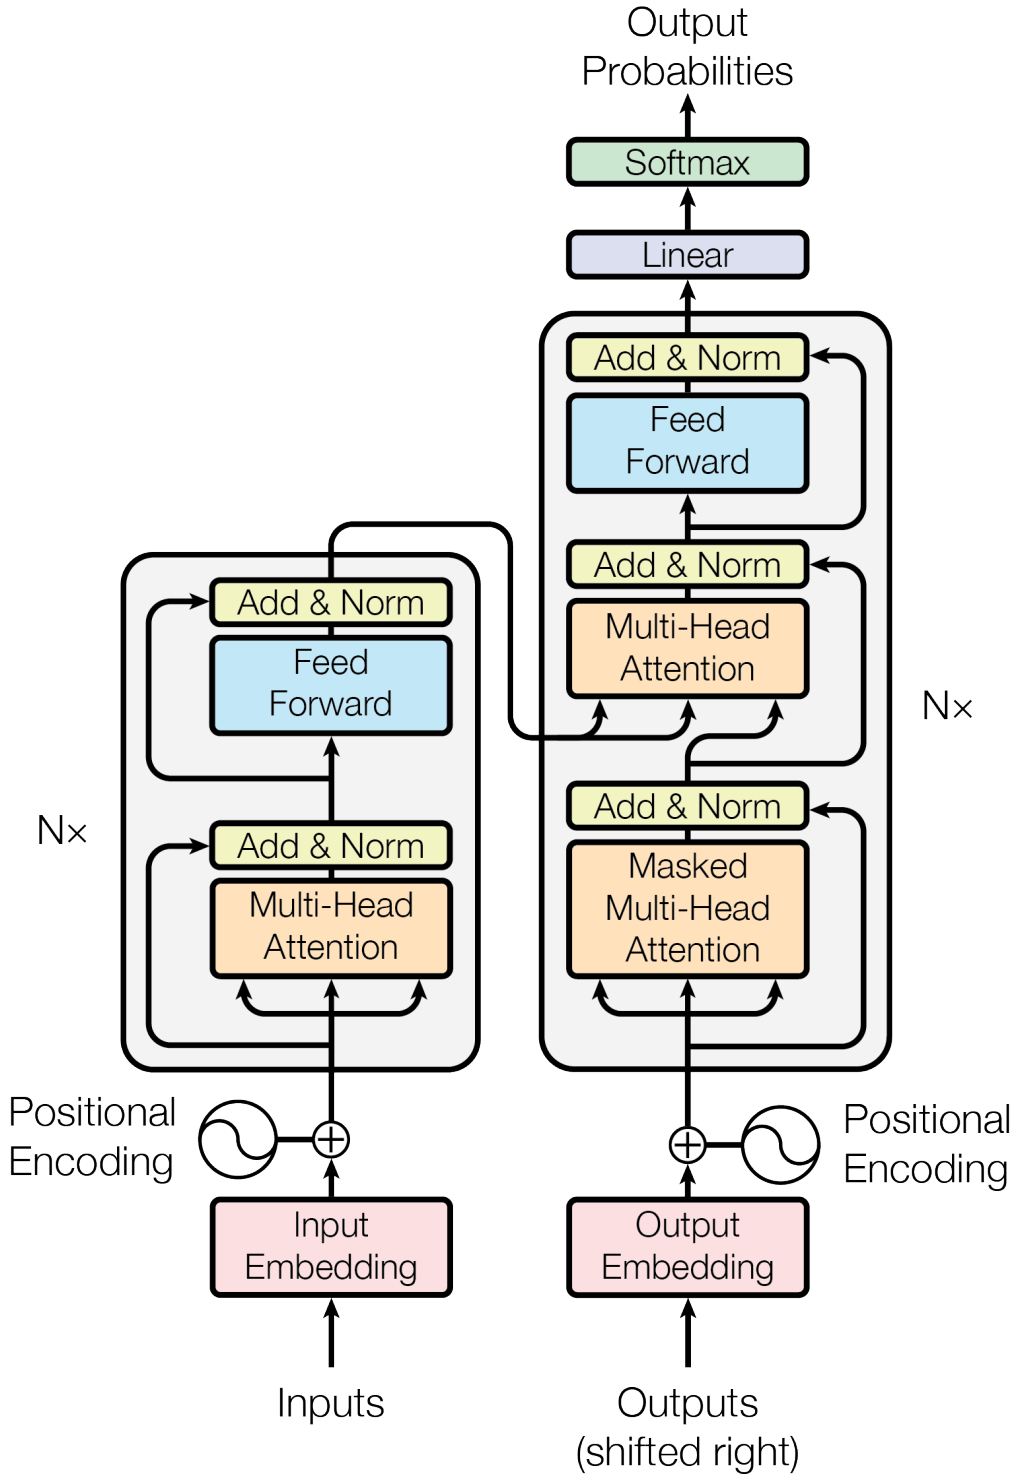
\includegraphics[width=0.5\textwidth]{Transformer model diagram}
\caption{Diagram depicting the architecture of the transformer model from \citet{AttentionIsAllYouNeed}.}
\end{figure}
\subsection{Problems solved by transformers}
The point of transformers was to overcome the problems faced by the previous state-of-the-art architectures while still including prominent aspects of the RNN and Convolutional Neural Network (CNN) models.

The RNN model has two notable weaknesses. First is its inability to learn long-term patterns, due to the exploding and vanishing gradient problems that occur during backpropagation.
Secondly, its recurrent connection is also a weakness. This is because it is not possible to compute the cell at time step $i$ until the cell at time step $i-1$ has been computed as information is propagated along a sequence.

In contrast, one of the benefits of CNNs is that they can be computed concurrently. However, unlike RNNs, they are unable to learn even short-term patterns. The size of the patterns they can learn is limited by their architecture.

Transformers attempt to feature the best of both techniques.
Transformers can model dependencies over the whole range of the input sequence as easily they can model neighboring sequences. And there are no recurrent connections, allowing efficient computation using parallelization. This is facilitated through the use of the self-attention mechanism.\cite{TransformersScratchPeterbloem}


\subsection{Self-attention Mechanism}
A self-attention mechanism is a sequence to sequence operation. This means that the input is a sequence of vectors $x_{1},x_{2},\ldots, x_{t}$, and the output is also a sequence of vectors $y_{1},y_{2},\ldots, y_{t}$.
These vectors all have dimension $k$.

To get the output vector $y_{i}$, the operation takes a weighted average over all input vectors.
$$
y_{i}=\sum_{j}w_{ij}x_{j}
$$
Here, $j$ indexes over the whole sequence, and the sum of all the weights in the sequence is one.
The weight $w_{ij}$ is derived from a function over $x_{i}$ and $x_{j}$.
This could, for example, be the dot product:
$$
w'_{ij}=x_{i}^Tx_{j}
$$
where $x_{i}$ is the input vector at the same position as the current output vector $y_{i}$.
The next output vector has a completely different series of dot products, and therefore a different weighted sum.

As the dot product can result in values between negative and positive infinity, the softmax activation function is used to map values to the interval $[0,1]$, and to ensure that they sum to $1$ over the entire sequence:
$$
w_{ij}=\frac{e^{w'_{ij}}}{\sum_{j}e^{w'_{ij}}}
$$
For maximum efficiency, computations are vectorized as much as possible. The resulting calculations become:
\begin{gather}
W'=X^TX\\
W=\text{softmax}(W')\\
Y^T=WX^T
\end{gather}\cite{TransformersScratchPeterbloem}


\subsection{How transformers work}
Transformers, as mentioned, primarily use self-attention. This forms the basis of the architecture.

There are several different variations of the transformer architecture, and the following is just one such variant.

First, the transformer block applies self-attention. Then it does layer normalization, after which it applies a feed forward network. The feed forward network here is a single MLP applied independently to each vector. And lastly, another layer normalization is applied.

The network may become permutation invariant, meaning the output will not change despite reordering. In the context of natural language processing, the ordering of the words in the input sentence would not matter. This can be detrimental to the training process, as it means the model is not learning the dependencies between words---positions matter. If every word in this paper were ordered alphabetically, it would not make much sense.

To solve this, one can use positional embeddings or positional encodings.

With positional embedding, the position of the word in the sentence is embedded. For this to work during training, sequences of every length would need to be seen, otherwise, the relevant positional embeddings do not get trained.

Positional encodings work in a similar fashion, except the positional vectors are not learned.
Instead, a function is chosen $f:\mathbb{N}\rightarrow\mathbb{R}^k$ that maps the positions to real-valued vectors. The network is left to figure out how to interpret these.\cite{TransformersScratchPeterbloem}


\section{Methodology}

\section{Experiment N \& Analysis}

\section{Conclusion}

%\section*{Acknowledgment}

\bibliographystyle{IEEEtranN}
\bibliography{bib/bib}

\appendix
%\input{appendix/...}

\end{document}